\documentclass[letterpaper,12pt,fleqn]{article}
\usepackage{matharticle}
\usetikzlibrary{arrows}
\pagestyle{empty}
\newcommand{\vx}{\vec{x}}
\newcommand{\vy}{\vec{y}}
\newcommand{\vz}{\vec{0}}
\newcommand{\va}{\vec{a}}
\newcommand{\vb}{\vec{b}}
\newcommand{\vc}{\vec{c}}
\newcommand{\vu}{\vec{u}}
\newcommand{\vv}{\vec{v}}
\newcommand{\norm}[1]{\|#1\|}
\begin{document}
\section*{Vectors}

\begin{definition}
  A \emph{vector} $\vx$ in 2D (or 3D) space is a quantity with both
  \emph{magnitude} and \emph{direction}. Vectors with the same magnitude and
  direction are considered equal, regardless of position.

  The zero vector, denoted $\vz$, is the vector with zero magnitude and no
  direction.
\end{definition}

Graphically, a non-zero vector is represented by a line terminated by an
arrow. The length of the line indicates the magnitude and the arrow indicates
the direction. When a vector is positioned with its tail at the origin, its
head coincides with a \emph{terminal point}:

\begin{center}
  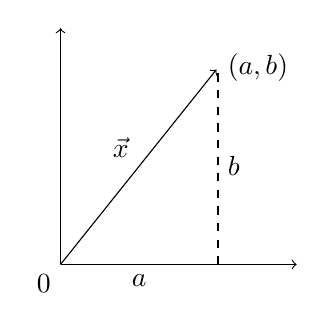
\begin{tikzpicture}
    \draw [->] (0,0) -- (3,0);
    \draw [->] (0,0) -- (0,3);
    \node [below left] at (0,0) {$0$};
    \node [scale=0.2] (x) at (2,2.5) {};
    \draw [->] (0,0) to node [above left] {$\vx$} (x)
    node [right] {$(a,b)$};
    \draw [dashed] (2,0) -- (x);
    \node [below] at (1,0) {$a$};
    \node [right] at (2,1.25) {$b$};
  \end{tikzpicture}
  
  $\vx=(a,b)$
\end{center}

Analytically, a vector is represented by the coordinates of its terminal point
(when originating from the origin), regardless of its actual position.

The zero vector has all zero components: $\vz=(0,0)$.

\begin{notation}
  The magnitude of a non-zero vector $\vx=(a,b)$, denoted $\norm{\vx}$, can be
  determined using the Pythagorean Theorem:
  \[\norm{\vx}=\sqrt{a^2+b^2}\]
  The zero vector has zero magnitude:
  \[\norm{\vz}=0\]
\end{notation}

\newpage

\subsection*{Vector Addition}

Graphically, vectors are added by placing them head-to-tail or by using the
parallelogram method:

\bigskip

\begin{center}
  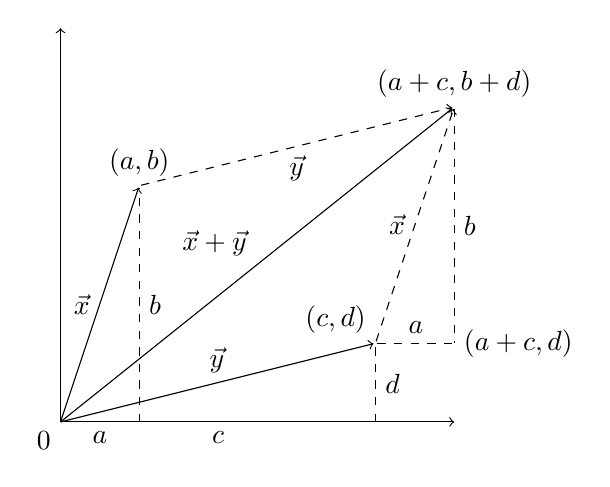
\begin{tikzpicture}
    \draw [->] (0,0) -- (5,0);
    \draw [->] (0,0) -- (0,5);
    \node [below left] at (0,0) {$0$};
    \node [scale=0.2] (xpy) at (5,4) {};
    \node [scale=0.2] (x) at (1,3) {};
    \node [scale=0.2] (y) at (4,1) {};
    \draw [->] (0,0) to node [left] {$\vx$} (x) node [above] {$(a,b)$};
    \draw [->] (0,0) to node [above] {$\vy$} (y)
    node [above left] {$(c,d)$};
    \draw [->] (0,0) to node [above left] {$\vx+\vy$} (xpy)
    node [above] {$(a+c,b+d)$};
    \draw [->,dashed] (x) to node [below] {$\vy$} (xpy);
    \draw [->,dashed] (y) to node [left] {$\vx$} (xpy);
    \draw [dashed] (y) to node [above] {$a$} (5,1);
    \draw [dashed] (xpy) to node [right] {$b$} (5,1) node [right] {$(a+c,d)$};
    \draw [dashed] (0,0) to node [below] {$a$} (1,0);
    \draw [dashed] (1,0) to node [right] {$b$} (x);
    \draw [dashed] (0,0) to node [below] {$c$} (4,0);
    \draw [dashed] (4,0) to node [right] {$d$} (y);
  \end{tikzpicture}
\end{center}

Analytically, vectors are added using component-wise addition of their terminal
points:
\begin{eqnarray*}
  \vx &=& (a,b) \\
  \vy &=& (c,d) \\
  \vx+\vy &=& (a+c,b+d)
\end{eqnarray*}

\begin{theorem}
  The zero vector acts as an additive identity:
  \[\vx+\vz=\vz+\vx=\vx\]
\end{theorem}

\begin{theproof}
  Let $\vx=(a,b)$ \\
  $\vx+\vz=(a,b)+(0,0)=(a+0,b+0)=(a,b)=\vx$ \\
  $\vz+\vx=(0,0)+(a,b)=(0+a,0+b)=(a,b)=\vx$
\end{theproof}

\newpage

\subsection*{Scalar Multiplication}

A vector can be multiplied by a real number, called a scalar, to change its
magnitude and/or direction:

\begin{center}
  \begin{tabular}{ll}
    $t>0$: & Increases/decreases the magnitude by a factor of $t$ \\
    $t=0$: & Results in the zero vector \\
    $t<0$: & Increases/decreases the magnitude by a factor of $\abs{t}$ and
    reverses the direction \\
  \end{tabular}
\end{center}

\bigskip

\begin{minipage}{4in}
  \begin{center}
    \begin{tikzpicture}
      \draw [->] (0,0) -- (5,0);
      \draw [->] (0,0) -- (0,5);
      \node [scale=0.2] (x) at (1.5,1.5) {};
      \node [scale=0.2] (tx) at (4,4) {};
      \draw [->] (0,0) to node [above left] {$\vx$} (x);
      \draw [->] (x) to node [above left] {$t\vx$} (tx) node [right] {$(x,y)$};
      \draw [dashed] (0,0) to node [below] {$a$} (1.5,0);
      \draw [dashed] (1.5,0) to node [right] {$b$} (x);
      \draw [dashed] (1.5,0) to node [below] {$ta$} (4,0);
      \draw [dashed] (4,0) to node [right] {$tb$} (tx);
    \end{tikzpicture}
  \end{center}
\end{minipage}
\begin{minipage}{3in}
  $\vx=(a,b)$

  \bigskip
  
  $\frac{\norm{\vx}}{t\norm{\vx}}=\frac{a}{x}\implies x=ta$

  \bigskip
    
  $\frac{\norm{\vx}}{t\norm{\vx}}=\frac{b}{y}\implies y=tb$

  \bigskip

  $t\vx=(ta,tb)$
\end{minipage}

\begin{definition}
  To say that two non-zero vectors $\vx$ and $\vy$ are \emph{parallel} means
  there exists some non-zero scalar $t$ such that $\vy=t\vx$. If $t>0$ then
  the vectors are in the same direction. If $t<0$ then the vectors are in
  reverse directions.
\end{definition}

\begin{notation}
  The vector $(-1)\vx$, denoted $-\vx$, is a vector parallel to $\vx$ with the
  same magnitude as $\vx$, but with the opposite direction of $\vx$.
\end{notation}

\begin{theorem}
  For every vector $\vx$, the vector $-\vx$ acts as an additive inverse:
  \[\vx+(-\vx)=(-\vx)+\vx=\vz\]
\end{theorem}

\begin{theproof}
  Let $\vx=(a,b)$ \\
  $-\vx=(-1)(a,b)=(-a,-b)$ \\
  $\vx+(-\vx)=(a,b)+(-a,-b)=(a-a,b-b)=(0,0)=\vz$ \\
  $(-\vx)+\vx=(-a,-b)+(a,b)=(-a+a,-b+b)=(0,0)=\vz$
\end{theproof}

\newpage

\subsection*{Vector Subtraction}

Using vector addition, inverses and identity, we can develop a notion of vector
subtraction:

\bigskip

\begin{center}
  \begin{tikzpicture}
    \draw [<->] (-5,0) -- (5,0);
    \draw [<->] (0,-5) -- (0,5);
    \node [scale=0.2] (x) at (1,3) {};
    \node [scale=0.2] (y) at (4,1) {};
    \draw [->] (0,0) to node [left] {$\vx$} (x) node [above] {$(a,b)$};
    \draw [->] (0,0) to node [above] {$\vy$} (y) node [right] {$(c,d)$};
    \draw [->] (y) to node [above] {$\vu$} (x);
    \node [scale=0.2] (my) at (-4,-1) {};
    \node [scale=0.2] (xmy) at (-3,2) {};
    \draw [->,dashed] (0,0) to node [below] {$-\vy$} (my)
    node [left] {$(-c,-d)$};
    \node [scale=0.2] (xmy) at (-3,2) {};
    \draw [->,dashed] (0,0) to node [above] {$\vu$} (xmy)
    node [left] {$(a-c,b-d)$};
    \draw [->,dashed] (my) to node [left] {$\vx$} (xmy);
    \draw [->,dashed] (x) to node [above] {$-\vy$} (xmy);
  \end{tikzpicture}
\end{center}

\begin{eqnarray*}
  \vy+\vu &=& \vx \\
  \vu &=& \vx-\vy \\
  \vu=(a,b)-(c,d) &=& (a-c,b-d)
\end{eqnarray*}

\newpage

\subsection*{Geometry}

\subsubsection*{Lines}

Problem: Find the vector equation for the line that passes through the terminal
points of two vectors $\va$ and $\vb$.

\bigskip

\begin{minipage}{3in}
  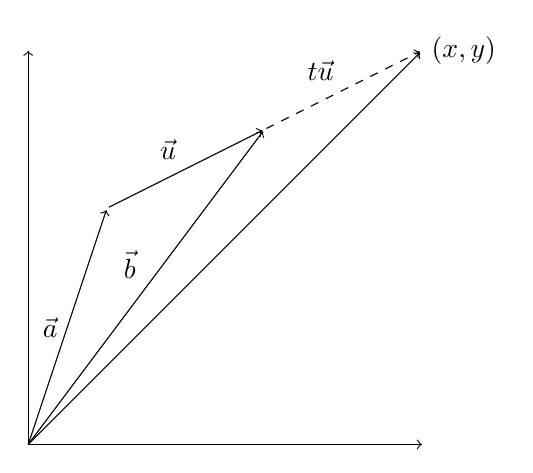
\begin{tikzpicture}
    \draw [->] (0,0) -- (5,0);
    \draw [->] (0,0) -- (0,5);
    \node [scale=0.2] (a) at (1,3) {};
    \node [scale=0.2] (b) at (3,4) {};
    \node [scale=0.2] (p) at (5,5) {};
    \draw [->] (0,0) to node [left] {$\vec{a}$} (a);
    \draw [->] (0,0) to node [above left] {$\vec{b}$} (b);
    \draw [->] (a) to node [above left] {$\vec{u}$} (b);
    \draw [->,dashed] (b) to node [above left] {$t\vec{u}$} (p);
    \draw [->] (0,0) -- (p) node [right] {$(x,y)$};
  \end{tikzpicture}
\end{minipage}
\begin{minipage}{3in}
  $\vec{u}=\vec{b}-\vec{a}$

  \bigskip

  $(x,y)=\vec{a}+t\vec{u}=\vec{a}+t(\vec{b}-\vec{a})$
\end{minipage}

\bigskip

\subsubsection*{Planes}

Problem: Find the vector equation for the plane that passes through the terminal
points of three non-colinear vectors $\va,\vb,$ and $\vc$.

\bigskip

\begin{minipage}{3in}
  \begin{tikzpicture}
    \draw [->] (0,0) -- (5,0);
    \draw [->] (0,0) -- (0,5);
    \draw [->] (0,0) -- (-2,-2);
    \node [scale=0.2] (a) at ({1/2},1) {};
    \draw [->] (0,0) to (a) node [above] {$\va$};
    \node [scale=0.2] (b) at (-1,2) {};
    \draw [->] (0,0) to node [left] {$\vb$} (b);
    \node [scale=0.2] (c) at (2,2) {};
    \draw [->] (0,0) to node [right] {$\vc$} (c);
    \draw [->] (a) to node [above] {$\vu$} (b);
    \draw [->] (a) to node [above] {$\vv$} (c);
    \node [scale=0.2] (su) at (-2,{8/3}) {};
    \draw [->,dashed] (b) to node [below] {$s\vu$} (su);
    \node [scale=0.2] (tv) at (3,{8/3}) {};
    \draw [->,dashed] (c) to node [below] {$t\vv$} (tv);
    \node [scale=0.2] (xy) at ({1/2},{13/3}) {};
    \draw [->,dashed] (su) to node [below] {$t\vv$} (xy);
    \draw [->,dashed] (tv) to node [below] {$s\vu$} (xy);
    \draw [->] (0,0) to (xy) node [above] {$(x,y)$};
  \end{tikzpicture}
\end{minipage}
\begin{minipage}{3in}
  $\vu=\vb-\va$ \\
  $\vv=\vc-\va$

  \bigskip

  $(x,y)=\va+s\vu+t\vv=\va+s(\vb-\va)+t(\vc-\va)$
\end{minipage}
\end{document}
